\begin{frame}[t]
\frametitle{Harnessing Parallelism: Challenges}
\framesubtitle{Trends in System Architecture}
    \begin{itemize}
        \item Frequencies have stopped increasing
        \item Memory costs are high
          \begin{itemize}
          \item Relatively low per core memory
          \end{itemize}
        \item Increasing heterogeneity
          \begin{itemize}
          \item Accelerators, SMT
          \end{itemize}
        \item Energy, power, and thermal considerations
        \item Frequent component failures
     \end{itemize}
\end{frame}

\begin{frame}[shrink]
\frametitle{Harnessing Parallelism: Challenges}
\framesubtitle{Trends in System Architecture}
  \begin{columns}
    \begin{column}{0.60\textwidth}
      \begin{itemize}
      \item However, compute resources are not faster cores, but \textbf{more cores}
      \item Unprecedented levels of available concurrency
        \begin{itemize}
        \item IBM BG/Q
          \begin{itemize}
          \item `Sequoia': 1,572,864 cores
          \item `Mira': 786,432 cores
          \end{itemize}
        \item Cray
          \begin{itemize}
          \item XE6 `Bluewaters`: $>$ 380,000 cores
          \item XK6 `Titan': 299,008 cores
          \end{itemize}
        \item K Supercomputer: 705,024 cores
        \end{itemize}
      \end{itemize}
    \end{column}
    \begin{column}{0.40\textwidth}
      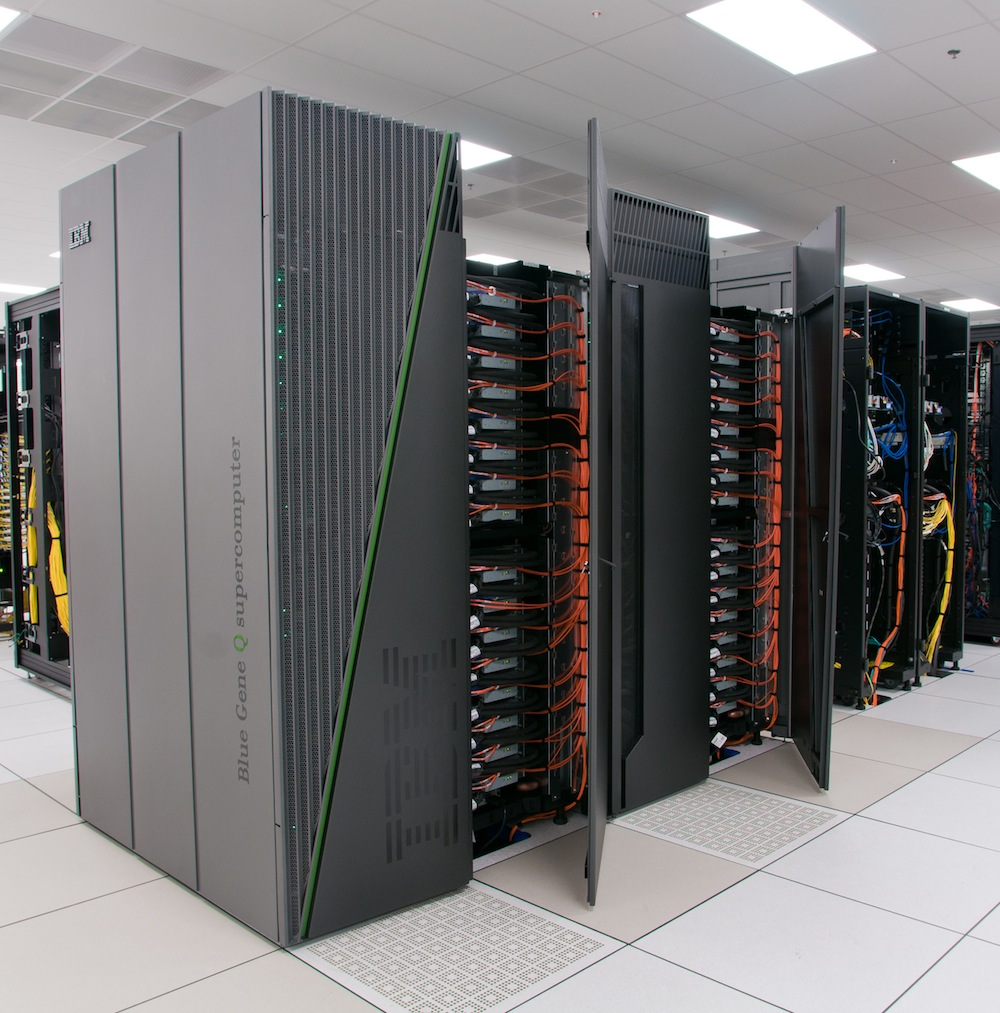
\includegraphics[width=1\textwidth]{figures/mira.jpg}
    \end{column}
  \end{columns}

  \begin{itemize}
    \item Mid-size clusters will be ubiquitous 
  \end{itemize}

    \pause
    \begin{block}{Implications}
        \begin{itemize}
            \item Each thread of execution has to:
                \begin{itemize}
                    \item operate on lesser data
                    \item wait relatively longer for remote data
                \end{itemize}
            \item Have to operate in \textbf{strong scaling} regime
            % Even if you don't do anything, an 8GB problem will have to run on
            % more cores a few years from now simply because there will be many
            % more cores for the same 8GB 
            % If a product has to stay ahead of the competition, it has to scale
            % the same problem to even more cores with time to run faster
        \end{itemize}
    \end{block}
\end{frame}

% \begin{frame}[t]
% \frametitle{Harnessing Parallelism: Challenges}
% \framesubtitle{Trends in System Architecture}
%     \begin{itemize}
%         \item Growing heterogeneity: Each thread of execution has different abilities
%             \begin{itemize}
%                 \item NUMA cores on each node
%                 \item Secondary threads in SMT can be less capable (IBM Power 7)
%                 \item Accelerators (NVIDIA / AMD GPUs, Intel MIC etc)
%                 \item Some cores run system daemons
%                 \item Combinations of above
%                     \begin{itemize}
%                         \item GPUs only on some nodes (BlueWaters: NCSA)
%                         \item MIC + SMT nodes (Stampede: TACC)
%                     \end{itemize}
%             \end{itemize}
%         \pause
%         \item Each architecture expects different treatment
%             \begin{itemize}
%                 \item GPUs expect evenly divided pieces
%                 \item SMT might expect uneven pieces (IBM Power7)
%             \end{itemize}
%     \end{itemize}
%     \pause
%     \begin{block}{Implications}
%         \begin{itemize}
%             \item Achieving load balance on such hardware is challenging
%             \item Minimizing idle time is extremely difficult
%         \end{itemize}
%     \end{block}
% \end{frame}


% \begin{frame}[t]
% \frametitle{Harnessing Parallelism: Challenges}
% \framesubtitle{Trends in System Architecture}
%   \begin{itemize}
%   \item Extracting performance on tighter power / energy budget
%   \item Hardware component failures / faults
%   \end{itemize}
% \end{frame}

% \begin{frame}[fragile]
% \frametitle{Harnessing Parallelism: Challenges}
% \framesubtitle{Application characteristics}
%   \begin{itemize}
%   \item Complex physics in multiple, interacting modules
%   \item Adaptive, spatial and temporal resolutions
%   \item Need for faster solutions (not just larger problems)
%   \end{itemize}
% \end{frame}

\begin{frame}[t]
\frametitle{Harnessing Parallelism: Challenges}
%\frametitle{Observations}
\framesubtitle{Next-generation Applications}
  \begin{itemize}
    \item Need for strong scaling
      \begin{itemize}
      \item faster solutions (not just larger problems)
      \end{itemize}
    \item Application Characteristics
    \begin{itemize}
      \item Multi-resolution
        \begin{itemize}
      \item Adaptive, spatial and temporal resolutions
      \item Dynamic/adaptive refinements: to handle application
        variation
        \end{itemize}
      \item Multi-module (multi-physics)
        \begin{itemize}
        \item Complex physics in multiple, interacting modules
        \end{itemize}
      \item Adapt to a volatile computational environment
      \item Exploit heterogeneous architecture
      \item Deal with thermal and energy considerations
    \end{itemize}
    \pause
    \item So? Consequences:
    \begin{itemize}
      \item Must support automated resource management
      \item Must support interoperability and parallel composition
    \end{itemize}
  \end{itemize}
\end{frame}

\begin{frame}[t]
\frametitle{Harnessing Parallelism: Challenges}
\framesubtitle{Programming Models: MPI}
  \begin{itemize}
    \item Highly successful
    \item Universally used
    \item Has supported application evolution from gigascale to petascale
  \end{itemize}
  \begin{itemize}
    \item Library
    \item Communication primitives
  \end{itemize}
  \begin{itemize}
    \item MPI does not directly support automated resource management
      (e.g. load balancing, fault tolerance, etc.)
  \end{itemize}
\end{frame}

% \begin{frame}[fragile]
% \frametitle{Harnessing Parallelism: Challenges}
% \framesubtitle{2D Jacobi Iterations: 5-point Stencil}
%    \begin{center} 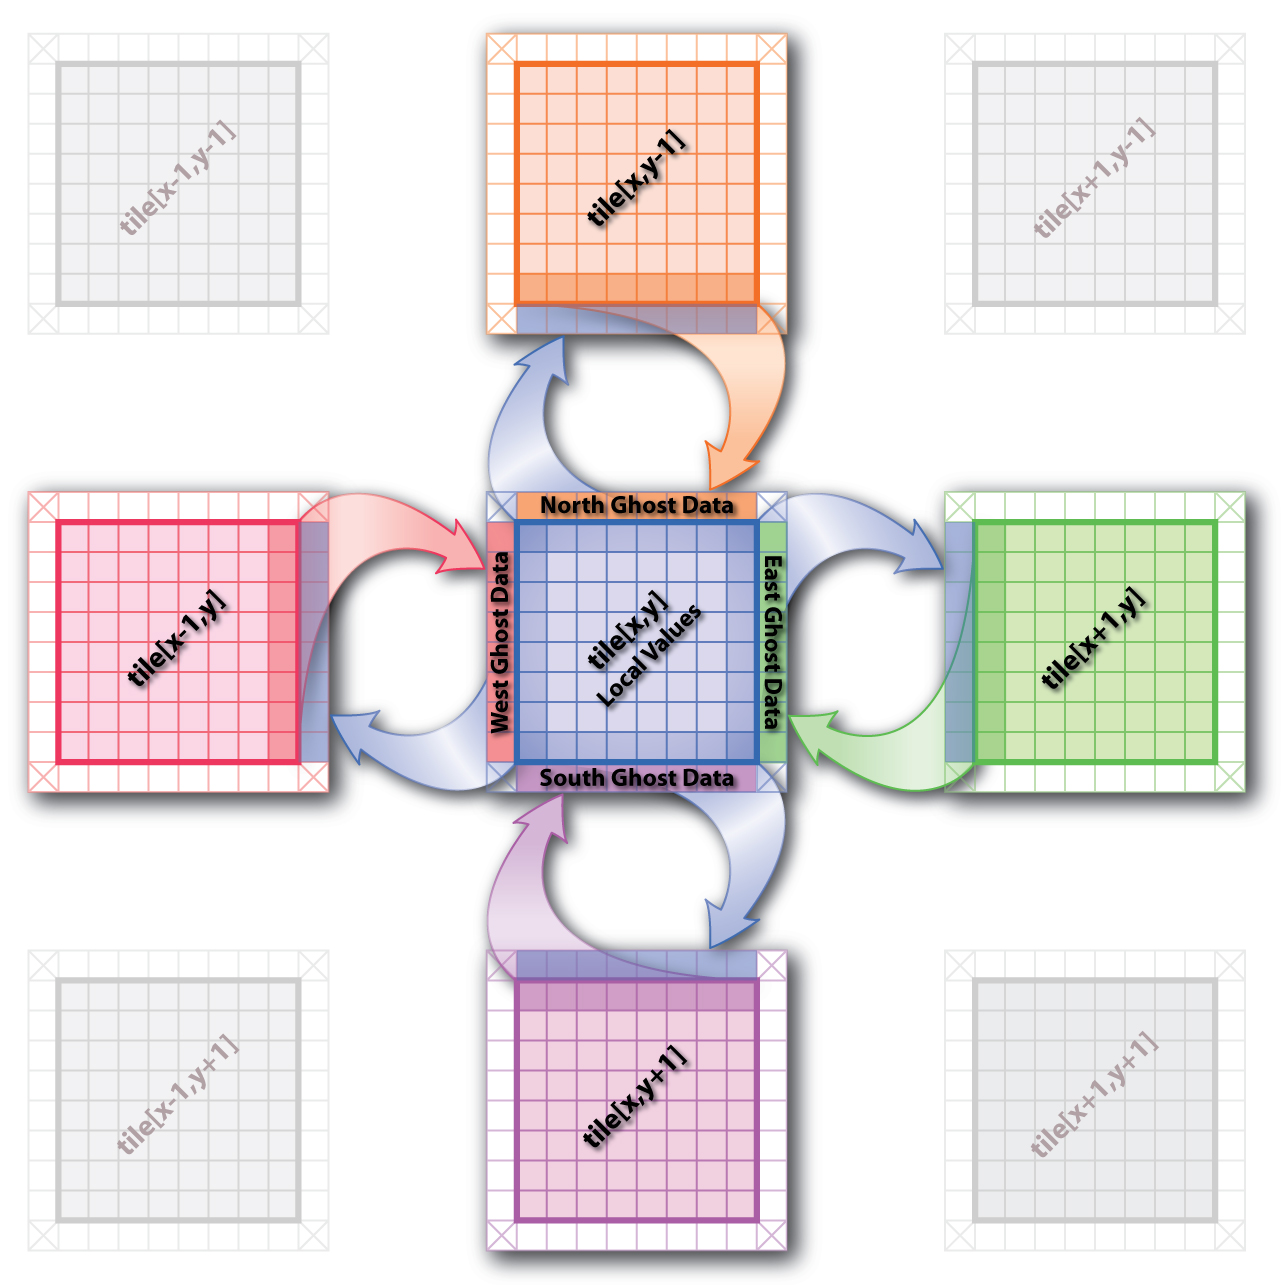
\includegraphics[width=0.6\textwidth]{figures/2DJacobi_NeighborComm.jpg} \end{center}
% \end{frame}


% \begin{frame}[fragile]
% \frametitle{Harnessing Parallelism: Challenges}
% \framesubtitle{2D Jacobi Iterations: No Overlap}
%     \lstinputlisting{code/jacobi2D-mpi.c}
% \end{frame}


% \begin{frame}[fragile, shrink]
% \frametitle{Harnessing Parallelism: Challenges}
% \framesubtitle{2D Jacobi Iterations: Some Overlap}
%     \lstinputlisting{code/jacobi2D-mpi-nonblocking.c}
% \end{frame}

\begin{frame}[fragile]
\frametitle{Harnessing Parallelism: Challenges}
\framesubtitle{Composing Independent Parallel Modules}
  \frametitle{Harnessing Parallelism}
  \framesubtitle{Composing Independent Parallel Modules}
  \begin{itemize}
    \item Sequential blocks (SEBs) in two modules can be partitioned in space
  \end{itemize}
  \begin{center}
    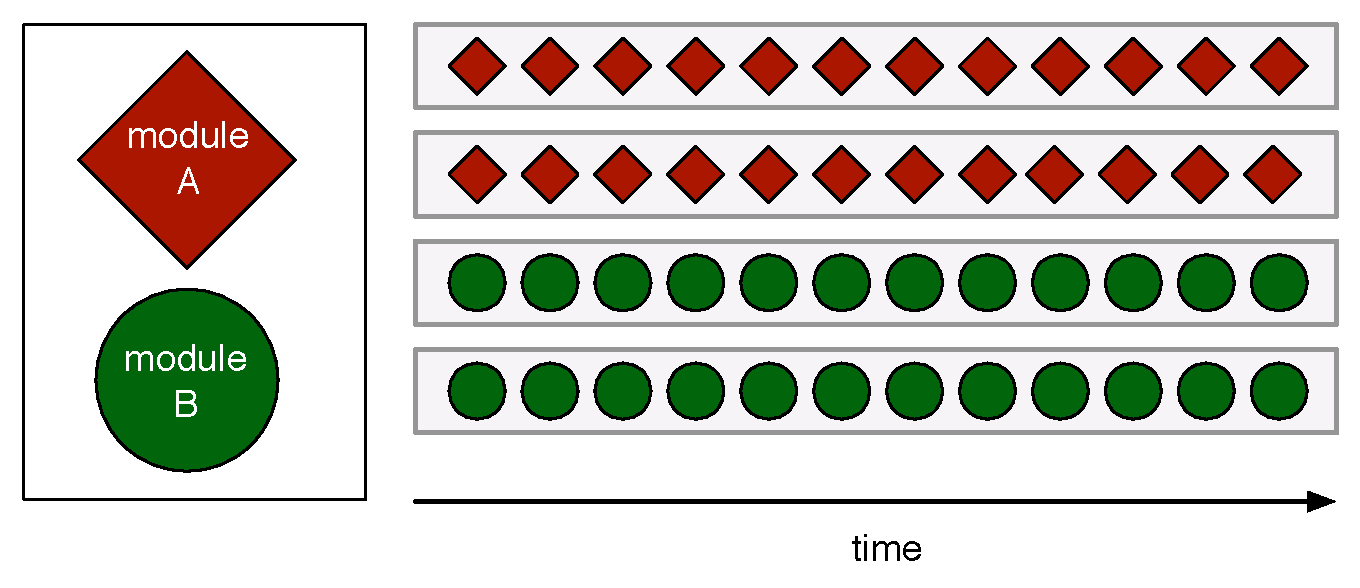
\includegraphics[width=0.8\textwidth]{figures/spaceDivision.pdf}
  \end{center}
\end{frame}

\begin{frame}[fragile]
\frametitle{Harnessing Parallelism: Challenges}
\framesubtitle{Composing Independent Parallel Modules}
  \begin{itemize}
    \item Sequential blocks (SEBs) in two modules can be partitioned in time
  \end{itemize}
  \begin{center}
    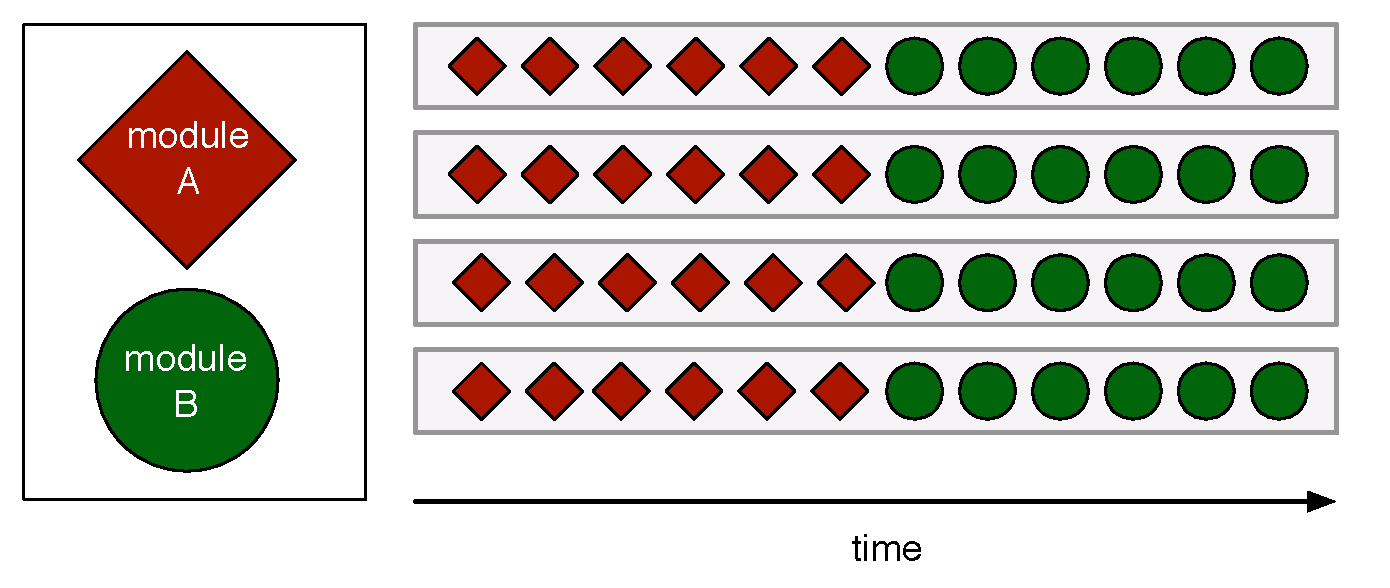
\includegraphics[width=0.8\textwidth]{figures/timeDivision.pdf}
  \end{center}
\end{frame}

\begin{frame}[fragile]
\frametitle{Stuff you already know}
\framesubtitle{Some issues with procedural code}

  \begin{columns}
    \begin{column}{0.4\textwidth}
      \lstinputlisting[basicstyle=\tiny]{code/jacobi2D-mpi.c}
    \end{column}
    \begin{column}{0.6\textwidth}
      \begin{itemize}
      \item Very similar to sequential code
      \item Tied to notion of communicating ranks
      \item Explicitly states order of computation and communication
      \item However no semantic connection between computation and its communication dependencies
      \end{itemize}
    \end{column}
  \end{columns}

\end{frame}

